\section{Decision Tree}\label{sec:dt}

\subsection{Giới thiệu về Decision Tree}
Cây quyết định (CART \cite{breiman1984}) chia không gian đặc trưng thành các vùng bằng chuỗi luật \textit{if--then}; mỗi lá dự đoán xác suất rời bỏ bằng tỉ lệ (có trọng số) của lớp rời bỏ trong vùng đó. Cây được xây dựng tham lam từ trên xuống: tại mỗi nút, thuật toán chọn đặc trưng và ngưỡng làm giảm nhiều nhất độ vẩn đục, đo bằng chỉ số Gini hoặc entropy ($p_k$: tỉ lệ lớp $k$ tại nút $S$):
\begin{equation}
    \text{Gini}(S) = 1 - \sum_{k} p_k^2, \qquad
    H(S) = -\sum_{k} p_k \log_2 p_k, \qquad
    \Delta I = I(S) - \tfrac{|S_L|}{|S|} I(S_L) - \tfrac{|S_R|}{|S|} I(S_R)
\end{equation}
Nếu không giới hạn, cây phát triển đến khi mọi lá thuần nhất và học thuộc dữ liệu huấn luyện; độ phức tạp được kiểm soát bằng \texttt{max\_depth} và \texttt{min\_samples\_leaf}.

\begin{table}[H]
\centering
\begin{adjustbox}{max width=\textwidth}
\begin{tabular}{|p{7cm}|p{7cm}|}
\hline
\textbf{Ưu điểm} & \textbf{Nhược điểm} \\
\hline
Dễ diễn giải, đọc trực tiếp được các luật & Phương sai cao, rất dễ overfit nếu không giới hạn \\
\hline
Không cần chuẩn hóa; tự học tương tác phi tuyến & Biên quyết định dạng bậc thang, xác suất thô \\
\hline
Huấn luyện và dự đoán rất nhanh & Cấu trúc thay đổi khi dữ liệu thay đổi nhỏ \\
\hline
\end{tabular}
\end{adjustbox}
\caption{Ưu và nhược điểm của Decision Tree}
\end{table}

\subsection{Mã nguồn và huấn luyện}
\begin{lstlisting}[style=pythonstyle, caption={Khởi tạo Decision Tree trong \texttt{src/models.py}}]
if model_name == "decision_tree":
    return DecisionTreeClassifier(
        class_weight=class_weight,   # "balanced" khi dung class weight
        random_state=random_state,
    )
\end{lstlisting}

\texttt{RandomizedSearchCV} (không gian tìm kiếm ở Mục~\ref{sec:exp4}) thử 50 tổ hợp trên 5 fold, chọn theo PR-AUC. Cấu hình tốt nhất: \texttt{criterion="entropy"}, \texttt{max\_depth=12}, \texttt{min\_samples\_leaf=51}. Cây cuối cùng (huấn luyện trên toàn bộ tập train) thực tế chỉ sâu 9 tầng và có 80 lá, vì ràng buộc \texttt{min\_samples\_leaf=51} khiến cây dừng tách trước khi đạt độ sâu 12.

\subsection{Kết quả và đánh giá}

\subsubsection{Kết quả cross-validation qua các giai đoạn}
\begin{table}[H]
\centering
\small
\begin{adjustbox}{max width=\textwidth}
\begin{tabular}{|l|c|c|c|c|c|c|}
\hline
\textbf{Cấu hình} & \textbf{Precision} & \textbf{Recall} & \textbf{F1} & \textbf{ROC-AUC} & \textbf{PR-AUC} & \textbf{F1 train} \\
\hline
Baseline & 0,489 & 0,496 & 0,492 & 0,654 & 0,377 & 0,997 \\
\hline
+ Class weight & 0,512 & 0,496 & 0,504 & 0,663 & 0,389 & 0,997 \\
\hline
+ Tuning & 0,508 & 0,799 & 0,621 & 0,830 & 0,630 & 0,646 \\
\hline
+ Ngưỡng 0,60 (out-of-fold) & 0,572 & 0,698 & \textbf{0,628} & 0,830 & 0,630 & -- \\
\hline
\end{tabular}
\end{adjustbox}
\caption{Decision Tree: kết quả validation (trung bình 5 fold) qua từng bước}
\end{table}

Decision Tree là mô hình hưởng lợi nhiều nhất từ tuning: F1 tăng 0,117 và PR-AUC tăng 0,242 so với class weight với tham số mặc định, cải thiện ở cả 5 fold. Ở cấu hình mặc định, cây học thuộc tập huấn luyện (F1 train 0,997) nên class weight gần như không có tác dụng; sau khi giới hạn kích thước lá, xác suất dự đoán mịn hơn và class weight mới đẩy được Recall từ 0,496 lên 0,799.

\subsubsection{Kết quả trên tập test}
\begin{table}[H]
\centering
\begin{minipage}[t]{0.56\textwidth}
\centering
\small
\begin{adjustbox}{max width=\textwidth}
\begin{tabular}{|l|c|c|c|c|}
\hline
\textbf{Lớp} & \textbf{Precision} & \textbf{Recall} & \textbf{F1-score} & \textbf{Support} \\
\hline
Không rời bỏ (0) & 0,89 & 0,80 & 0,84 & 1.035 \\
\hline
Rời bỏ (1) & 0,56 & 0,72 & 0,63 & 374 \\
\hline
Accuracy & & & 0,78 & 1.409 \\
\hline
Macro avg & 0,72 & 0,76 & 0,73 & 1.409 \\
\hline
Weighted avg & 0,80 & 0,78 & 0,78 & 1.409 \\
\hline
\end{tabular}
\end{adjustbox}
\caption{Decision Tree: kết quả phân loại trên tập test (ngưỡng 0,60; ROC-AUC 0,835; PR-AUC 0,624)}
\end{minipage}\hfill
\begin{minipage}[t]{0.42\textwidth}
\centering
\small
\begin{adjustbox}{max width=\textwidth}
\begin{tabular}{|c|c|c|c|}
\cline{3-4}
\multicolumn{2}{c|}{} & \multicolumn{2}{c|}{\textbf{Dự đoán}} \\
\cline{3-4}
\multicolumn{2}{c|}{} & Không rời bỏ & Rời bỏ \\
\hline
\multirow{2}{*}{\textbf{Thực tế}} & Không rời bỏ & \cellcolor{blue!30}823 & 212 \\
\cline{2-4}
 & Rời bỏ & 105 & \cellcolor{blue!30}269 \\
\hline
\end{tabular}
\end{adjustbox}
\caption{Decision Tree: Confusion Matrix trên tập test}
\end{minipage}
\end{table}

So với lần đánh giá test đầu tiên (tham số mặc định, không xử lý mất cân bằng, ngưỡng 0,5), số khách hàng rời bỏ được phát hiện tăng từ 186 lên 269 (Recall 0,497 lên 0,719), F1 từ 0,492 lên 0,629 và ROC-AUC từ 0,654 lên 0,835.

\subsubsection{Cấu trúc cây quyết định}
\begin{figure}[H]
\centering
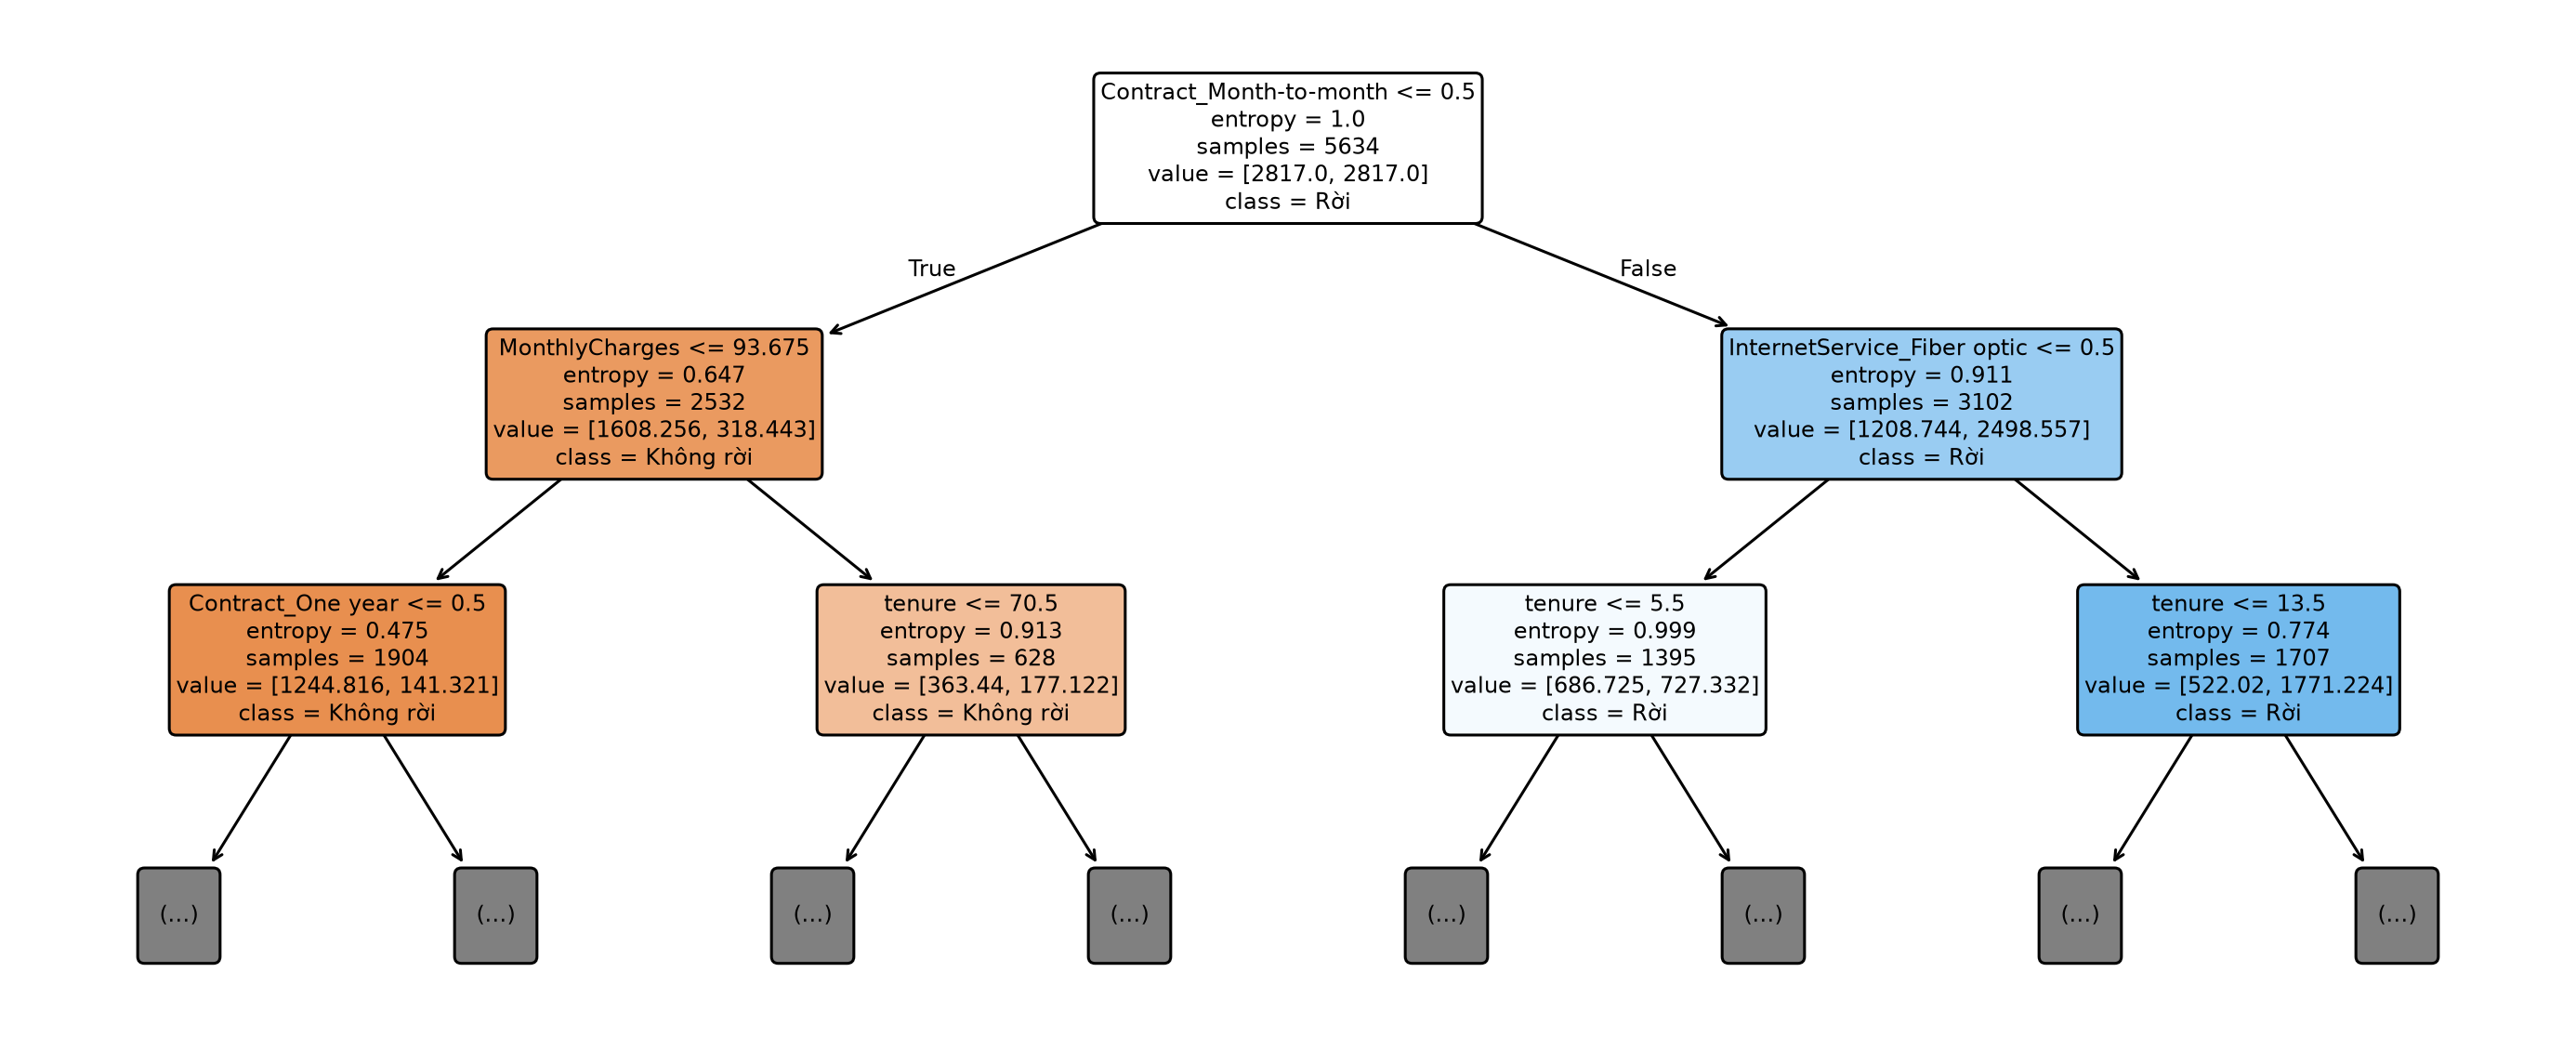
\includegraphics[width=0.9\textwidth]{img/dt_structure.png}
\caption{Ba tầng đầu của cây quyết định đã tuning. \texttt{value} là tổng trọng số (sau class weight) của hai lớp [không rời bỏ, rời bỏ]; màu cam: nghiêng về không rời bỏ, màu xanh: nghiêng về rời bỏ.}
\label{fig:dt_structure}
\end{figure}

Các luật ở những tầng đầu khớp với EDA:
\begin{itemize}
    \item \textbf{Nút gốc} tách theo \texttt{Contract\_Month-to-month}: nhánh hợp đồng theo tháng (3.102 khách hàng) nghiêng hẳn về rời bỏ, nhánh hợp đồng dài hạn (2.532 khách hàng) nghiêng về ở lại.
    \item \textbf{Với hợp đồng theo tháng}, cây tiếp tục tách theo \texttt{InternetService\_Fiber optic}, rồi theo \texttt{tenure}: khách hàng dùng Fiber optic và có \texttt{tenure} $\le 13{,}5$ tháng là nhóm rủi ro cao nhất.
    \item \textbf{Với hợp đồng dài hạn}, cây tách theo \texttt{MonthlyCharges} $\le 93{,}7$ USD; khách hàng hợp đồng dài hạn và cước thấp gần như không rời bỏ.
\end{itemize}

\subsubsection{Feature Importance}
\begin{figure}[H]
\centering
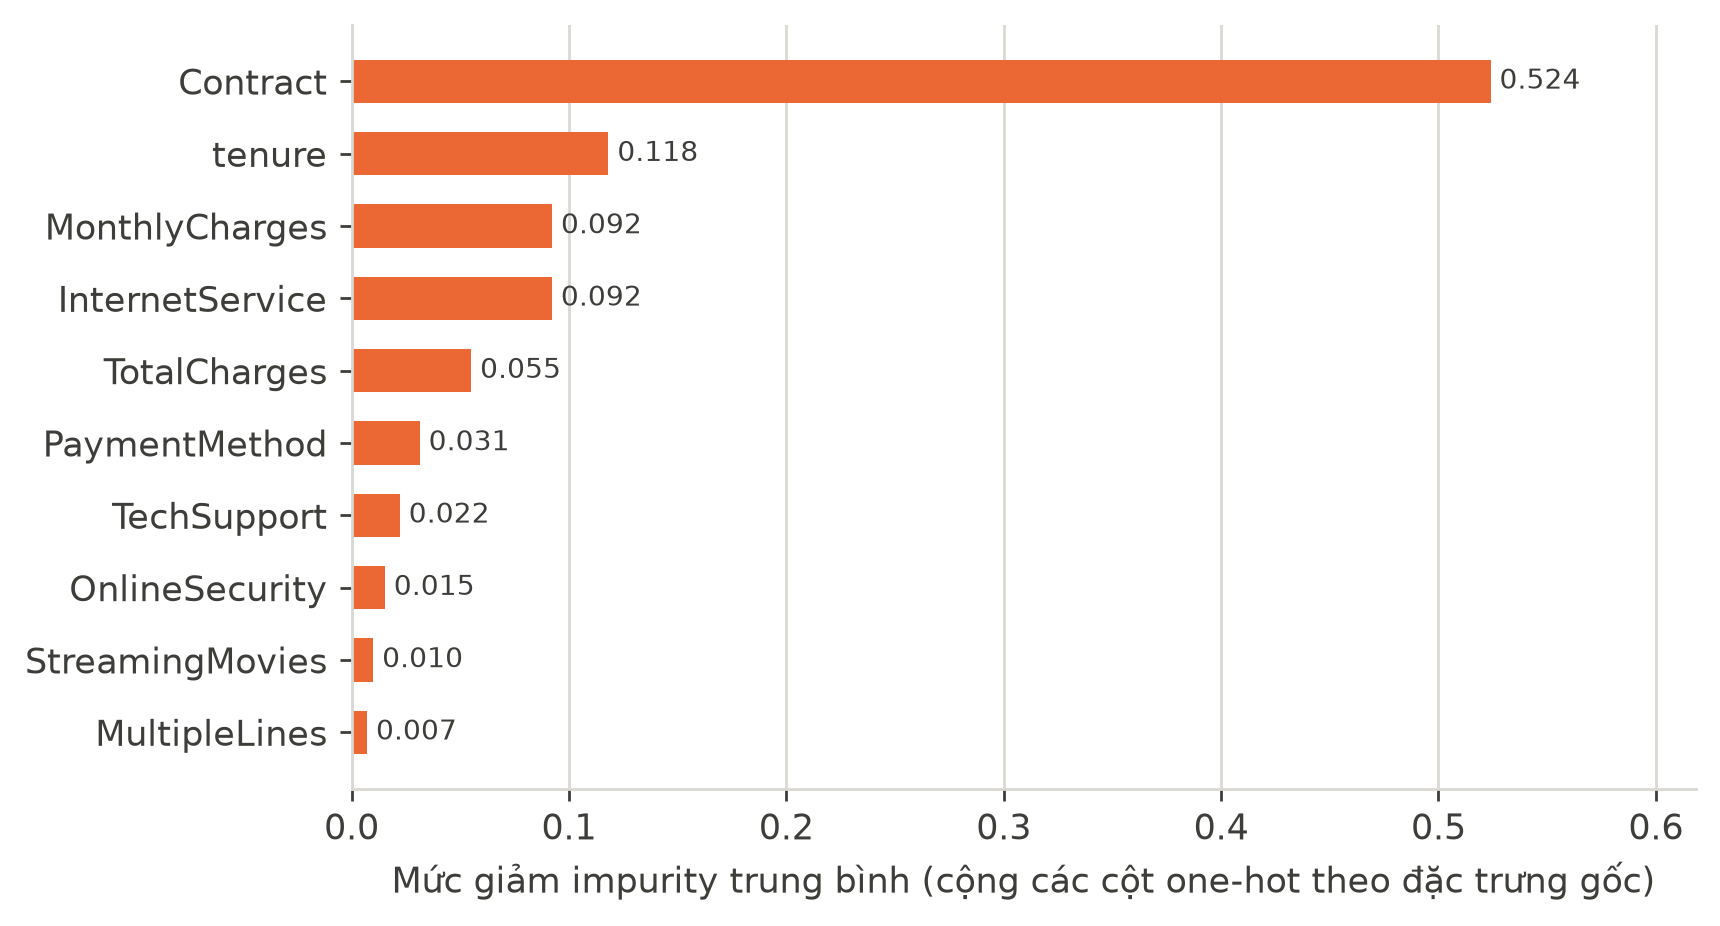
\includegraphics[width=0.75\textwidth]{img/importance_decision_tree.png}
\caption{Decision Tree: impurity importance của 10 đặc trưng gốc quan trọng nhất}
\end{figure}

\texttt{Contract} chiếm 52\% tổng mức giảm entropy (chủ yếu từ nút gốc), tiếp theo là \texttt{tenure} (12\%), \texttt{MonthlyCharges} và \texttt{InternetService} (mỗi đặc trưng 9\%). Các đặc trưng nhân khẩu học gần như không được dùng.

\subsubsection{Nhận xét và đánh giá}
\textbf{Điểm mạnh}
\begin{itemize}
    \item Sau tuning, Decision Tree từ mô hình kém nhất (F1 0,492) trở nên cạnh tranh với các mô hình phức tạp hơn: F1 test 0,629, chỉ kém XGBoost 0,005.
    \item Dễ diễn giải nhất: có thể trình bày trực tiếp cho bộ phận kinh doanh dưới dạng các luật như ``hợp đồng theo tháng + Fiber optic + mới dùng dưới 14 tháng $\Rightarrow$ rủi ro cao''.
    \item Kết quả test khớp với cross-validation (F1 0,628 so với 0,629; PR-AUC 0,630 so với 0,624).
\end{itemize}

\textbf{Hạn chế}
\begin{itemize}
    \item ROC-AUC và PR-AUC thấp nhất trong bốn mô hình (0,835 và 0,624): với 80 lá, xác suất dự đoán chỉ nhận tối đa 80 giá trị khác nhau nên khả năng xếp hạng khách hàng kém hơn các mô hình ensemble.
    \item Rất nhạy với siêu tham số: ở cấu hình mặc định mô hình overfit nặng (F1 train 0,997, ROC-AUC validation 0,654).
    \item Cây đơn có phương sai cao, cấu trúc có thể thay đổi khi dữ liệu huấn luyện thay đổi.
\end{itemize}

\textbf{Hướng cải thiện}
\begin{enumerate}
    \item Thử cắt tỉa theo độ phức tạp chi phí (\texttt{ccp\_alpha}) thay cho giới hạn độ sâu.
    \item Dùng Decision Tree như công cụ diễn giải (cây nông 3--4 tầng) bên cạnh một mô hình ensemble dùng để dự đoán.
\end{enumerate}
